%%%% Paramétrage du TD %%%%
%\def\xxnumchapitre{Chapitre 2 \vspace{.2cm}}
%\def\xxchapitre{\hspace{.12cm} Représentation des nombres}

\def\xxcompetences{%
\textsl{%
\textbf{Savoirs et compétences :}\\
\vspace{-.4cm}
\begin{itemize}[label=\ding{112},font=\color{bleuxp}] 
\item .
%\item \textit{Mod3.C2 : } pôles dominants et réduction de l’ordre du modèle : principe, justification
%\item \textit{Res2.C4 : } stabilité des SLCI : définition entrée bornée -- sortie bornée (EB -- SB)	
%\item \textit{Res2.C5 : } stabilité des SLCI : équation caractéristique	
%\item \textit{Res2.C6 : } stabilité des SLCI : position des pôles dans le plan complexe
%\item \textit{Res2.C7 : } stabilité des SLCI : marges de stabilité (de gain et de phase)
\end{itemize}
}}


\def\xxfigures{
%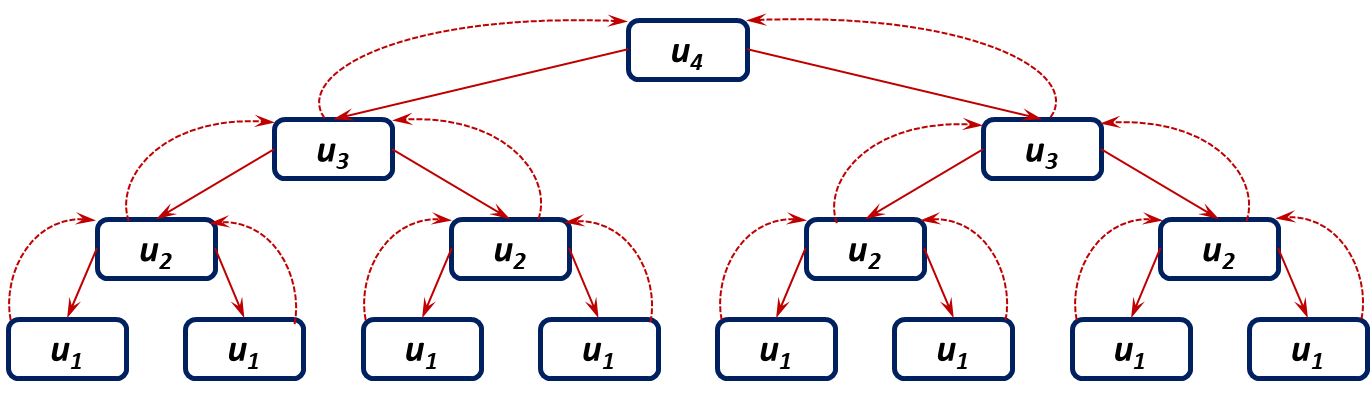
\includegraphics[width=3cm]{fig_01}\\
%\textit{}
}%figues de la page de garde

\def\xxtitreexo{Applications -- Bases}
\def\xxsourceexo{}
\def\xxactivite{{ Application 01} \ifprof  -- Corrigé \else \fi}

%\iflivret
\input{\repRel/Style/pagegarde_TD}
%\else
%\pagestyle{empty}


%%%%%%%% PAGE DE GARDE COURS
\ifcours
\begin{tikzpicture}[remember picture,overlay]
\node at (current page.north west)
{\begin{tikzpicture}[remember picture,overlay]
\node[anchor=north west,inner sep=0pt] at (0,0) {\includegraphics[width=\paperwidth]{\thechapterimage}};
\draw[anchor=west] (-2cm,-8cm) node [line width=2pt,rounded corners=15pt,draw=ocre,fill=white,fill opacity=0.6,inner sep=40pt]{\strut\makebox[22cm]{}};
\draw[anchor=west] (1cm,-8cm) node {\huge\sffamily\bfseries\color{black} %
\begin{minipage}{1cm}
\rotatebox{90}{\LARGE\sffamily\textsc{\color{ocre}\textbf{\xxnumpartie}}}
\end{minipage} \hfill
\begin{minipage}[c]{14cm}
\begin{titrepartie}
\begin{flushright}
\renewcommand{\baselinestretch}{1.1} 
\Large\sffamily\textsc{\textbf{\xxpartie}}
\renewcommand{\baselinestretch}{1} 
\end{flushright}
\end{titrepartie}
\end{minipage} \hfill
\begin{minipage}[c]{3.5cm}
{\large\sffamily\textsc{\textbf{\color{ocre} \discipline}}}
\end{minipage} 
 };
\end{tikzpicture}};
\end{tikzpicture}


\begin{tikzpicture}[overlay]
\node[shape=rectangle, 
      rounded corners = .25 cm,
	  draw= ocre,
	  line width=2pt, 
	  fill = ocre!10,
	  minimum width  = 2.5cm,
	  minimum height = 3cm,] at (18cm,0) {};
\node at (17.7cm,0) {\rotatebox{90}{\textbf{\Large\color{ocre}{\classe}}}};
%{};
\end{tikzpicture}

\vspace{3.5cm}

\begin{tikzpicture}[remember picture,overlay]
\draw[anchor=west] (-2cm,-6cm) node {\huge\sffamily\bfseries\color{black} %
\begin{minipage}{2cm}
\begin{center}
\LARGE\sffamily\textsc{\color{ocre}\textbf{\xxactivite}}
\end{center}
\end{minipage} \hfill
\begin{minipage}[c]{15cm}
\begin{titrechapitre}
\renewcommand{\baselinestretch}{1.1} 
\Large\sffamily\textsc{\textbf{\xxnumchapitre}}

\Large\sffamily\textsc{\textbf{\xxchapitre}}
\vspace{.5cm}

\renewcommand{\baselinestretch}{1} 
\normalsize\normalfont
\xxcompetences
\end{titrechapitre}
\end{minipage}  };
\end{tikzpicture}
\vfill

\begin{flushright}
\begin{minipage}[c]{.3\linewidth}
\begin{center}
\xxfigures
\end{center}
\end{minipage}\hfill
\begin{minipage}[c]{.6\linewidth}
\startcontents
\printcontents{}{1}{}
\end{minipage}
\end{flushright}

\begin{tikzpicture}[remember picture,overlay]
\draw[anchor=west] (4.5cm,-.7cm) node {
\begin{minipage}[c]{.2\linewidth}
\begin{flushright}

\includegraphics[width=2cm]{png/logoCC}
\end{flushright}
\end{minipage}
\begin{minipage}[c]{.2\linewidth}
\textsl{\xxauteur} \\
\textsl{\classe}
\end{minipage}
 };
\end{tikzpicture}
\newpage
\pagestyle{fancy}

\newpage
\pagestyle{fancy}

\else
\fi


%%%%%%%% PAGE DE GARDE TD
\iftd
%\begin{tikzpicture}[remember picture,overlay]
%\node at (current page.north west)
%{\begin{tikzpicture}[remember picture,overlay]
%\draw[anchor=west] (-2cm,-3.25cm) node [line width=2pt,rounded corners=15pt,draw=ocre,fill=white,fill opacity=0.6,inner sep=40pt]{\strut\makebox[22cm]{}};
%\draw[anchor=west] (1cm,-3.25cm) node {\huge\sffamily\bfseries\color{black} %
%\begin{minipage}{1cm}
%\rotatebox{90}{\LARGE\sffamily\textsc{\color{ocre}\textbf{\xxnumpartie}}}
%\end{minipage} \hfill
%\begin{minipage}[c]{13.5cm}
%\begin{titrepartie}
%\begin{flushright}
%\renewcommand{\baselinestretch}{1.1} 
%\Large\sffamily\textsc{\textbf{\xxpartie}}
%\renewcommand{\baselinestretch}{1} 
%\end{flushright}
%\end{titrepartie}
%\end{minipage} \hfill
%\begin{minipage}[c]{3.5cm}
%{\large\sffamily\textsc{\textbf{\color{ocre} \discipline}}}
%\end{minipage} 
% };
%\end{tikzpicture}};
%\end{tikzpicture}

%%%%%%%%%% PAGE DE GARDE TD %%%%%%%%%%%%%%%
%\begin{tikzpicture}[overlay]
%\node[shape=rectangle, 
%      rounded corners = .25 cm,
%	  draw= ocre,
%	  line width=2pt, 
%	  fill = ocre!10,
%	  minimum width  = 2.5cm,
%	  minimum height = 2.5cm,] at (18.5cm,0) {};
%\node at (17.7cm,0) {\rotatebox{90}{\textbf{\Large\color{ocre}{\classe}}}};
%%{};
%\end{tikzpicture}

% PARTIE ET CHAPITRE
%\begin{tikzpicture}[remember picture,overlay]
%\draw[anchor=west] (-1cm,-2.1cm) node {\large\sffamily\bfseries\color{black} %
%\begin{minipage}[c]{15cm}
%\begin{flushleft}
%\xxnumchapitre \\
%\xxchapitre
%\end{flushleft}
%\end{minipage}  };
%\end{tikzpicture}

% Bandeau titre exo
\begin{tikzpicture}[remember picture,overlay]
\draw[anchor=west] (-2cm,-4cm) node {\huge\sffamily\bfseries\color{black} %
\begin{minipage}{5cm}
\begin{center}
\LARGE\sffamily\color{ocre}\textbf{\textsc{\xxactivite}}

\begin{center}
\xxfigures
\end{center}

\end{center}
\end{minipage} \hfill
\begin{minipage}[c]{12cm}
\begin{titrechapitre}
\renewcommand{\baselinestretch}{1.1} 
\large\sffamily\textbf{\textsc{\xxtitreexo}}

\small\sffamily{\textbf{\textit{\color{black!70}\xxsourceexo}}}
\vspace{.5cm}

\renewcommand{\baselinestretch}{1} 
\normalsize\normalfont
\xxcompetences
\end{titrechapitre}
\end{minipage}  };
\end{tikzpicture}
\else
\fi


%%%%%%%% PAGE DE GARDE FICHE
\iffiche
\begin{tikzpicture}[remember picture,overlay]
\node at (current page.north west)
{\begin{tikzpicture}[remember picture,overlay]
\draw[anchor=west] (-2cm,-3.25cm) node [line width=2pt,rounded corners=15pt,draw=ocre,fill=white,fill opacity=0.6,inner sep=40pt]{\strut\makebox[22cm]{}};
\draw[anchor=west] (1cm,-3.25cm) node {\huge\sffamily\bfseries\color{black} %
\begin{minipage}{1cm}
\rotatebox{90}{\LARGE\sffamily\textsc{\color{ocre}\textbf{\xxnumpartie}}}
\end{minipage} \hfill
\begin{minipage}[c]{14cm}
\begin{titrepartie}
\begin{flushright}
\renewcommand{\baselinestretch}{1.1} 
\large\sffamily\textsc{\textbf{\xxpartie} \\} 

\vspace{.2cm}

\normalsize\sffamily\textsc{\textbf{\xxnumchapitre -- \xxchapitre}}
\renewcommand{\baselinestretch}{1} 
\end{flushright}
\end{titrepartie}
\end{minipage} \hfill
\begin{minipage}[c]{3.5cm}
{\large\sffamily\textsc{\textbf{\color{ocre} \discipline}}}
\end{minipage} 
 };
\end{tikzpicture}};
\end{tikzpicture}


\begin{tikzpicture}[overlay]
\node[shape=rectangle, 
      rounded corners = .25 cm,
	  draw= ocre,
	  line width=2pt, 
	  fill = ocre!10,
	  minimum width  = 2.5cm,
	  minimum height = 2.5cm,] at (18.5cm,0.5cm) {};
%	  minimum height = 2.5cm,] at (18.5cm,0cm) {};
\node at (17.7cm,0.5) {\rotatebox{90}{\textsf{\textbf{\large\color{ocre}{\classe}}}}};
%{};
\end{tikzpicture}

\else
\fi



%\fi

\setlength{\columnseprule}{.1pt}

\pagestyle{fancy}
\thispagestyle{plain}


\vspace{4.5cm}

\def\columnseprulecolor{\color{bleuxp}}
\setlength{\columnseprule}{0.4pt} 

%%%%%%%%%%%%%%%%%%%%%%%




\ifprof
\vspace{1cm}
\else
\begin{multicols}{2}
\fi

\exer{}
\setcounter{numques}{0}

On considère la fonction \texttt{mystere} suivante, qui étant donnés deux entiers \texttt{x} et \texttt{x}, renvoie un autre
entier.
\begin{lstlisting}
def mystere(x :int, y :int) -> int :
    a=0
    while y>0 :
        if y%2==1 :
            a=a+x
        x=x+x
        y=y//2
    return(a)
\end{lstlisting}

\question{Recopier et compléter les tableaux suivants donnant l’évolution des variables \texttt{x}, \texttt{y} et \texttt{a} ainsi
que de la quantité \texttt{a+x*y} lors des appels \texttt{f(7,20)} et \texttt{f(3,85)}.}
\ifprof
\begin{corrige}
\begin{center}
\begin{tabular}{l c c c c }
\hline
Pour \texttt{mystere(7,20)} & x  & y & a & $a+x*y$ \\
\hline
\hline
Fin du premier tour de boucle     &14 & 10 & 0 & 140 \\ \hline
Fin du deuxième tour de boucle  & 28 & 5 & 0 & 140\\ \hline
Fin du troisième tour de boucle   & 56 & 2 & 28 & 140\\ \hline
Fin du quatrième tour de boucle &  112 & 1 & 28 & 140\\ \hline
Fin du cinquième tour de boucle & 224 & 0 & 140 & 140\\ \hline
\end{tabular}
\end{center}
\end{corrige}
\else
\fi

\question{Montrer que la fonction \texttt{mystere} termine.}
\ifprof
\begin{corrige}
\begin{tabular}{l c c c c }
\hline
Pour \texttt{mystere(3,85)} & x  & y & a & $a+x*y$ \\
\hline
\hline
Fin du premier tour de boucle     & 6    & 42 & 3     & 255\\ \hline
Fin du deuxième tour de boucle & 12   & 21 &3      & 255 \\ \hline
Fin du troisième tour de boucle  & 24   & 10 & 15   & 255 \\ \hline
Fin du quatrième tour de boucle & 48   & 5 & 15     & 255 \\ \hline
Fin du cinquième tour de boucle & 96   & 2  & 63    & 255 \\ \hline
Fin du sixième tour de boucle     & 192  & 1 & 63    & 255 \\ \hline
Fin du septième tour de boucle   & 384 & 0 &  255 & 255 \\ \hline
\end{tabular}
\end{corrige}
\else
\fi

\question{Conjecturer la valeur de \texttt{mystere(x,y)} et démontrer cette conjecture à l’aide d’un invariant
de boucle bien choisi (on pourra appeler $x_i$ , $y_i$ et $a_i$ les valeurs respectives de $x$, $y$ et $a$
à l’entrée du \ieme  $i\geq 0$ tour de boucle).}
\ifprof
\begin{corrige}
On conjecture que \texttt{mystere(x,y)} renvoie $xy$.
Considérons l'invariant : << à l’entrée du i\ieme tour de boucle, $a_i+x_i y_i = x *y $>>.
\begin{itemize}
\item Pour$ i=0$, on a $a_0 = 0$, $x_0 = x$, $y_0 = y$ donc $a_0 + x_0 y_0 = xy$.
\item Soit  $i\geq 0$. On suppose qu’au rang $i$ , on a $a_i x_i y_i =xy$.
\begin{itemize}
\item Soit $y_i$  pair alors $x_{i+1}=x_i+x_i = 2x_i$, $y_{i+1}=\dfrac{y_i}{2}$ et $a_{i+1}=a_i +x_i$.
\begin{itemize}
\item Donc $a_{i+1}+x_{i+1}y_{i+1}=a_i+2x_i\dfrac{y_i}{2} = a_i +x_iy_i = xy$.
\end{itemize}
\item Soit $y_i$ impair alors $x_{i+1}=x_i + x_i = 2 x_i$, $y_{i+1}=\dfrac{y_i -1}{2}$ et $a_{i+1}=a_i x_i$.
\begin{itemize}
\item Donc $a_{i+1}+x_{i+1}y_{i+1}=a_i+x_i+2 x_i \dfrac{y_i}{2} = a_i +x_i+x_i\left( y_i -1 \right) = xy$.
\end{itemize}
\end{itemize}
\end{itemize}

Cela prouve l’invariant de boucle.
À la dernière étape, on a $a_{i-1}+x_{i-1}y_{i-1}=xy$ avec $y{i-1}=1$ donc $y_i = 0$, $a_i=a_{i-1}+x_{i-1}y_{i-1} = xy$ donc \texttt{mystere(x,y)} renvoie bien $x.y$ ce qui achève la correction de programme.

\end{corrige}
\else
\fi

\exer{}
\setcounter{numques}{0}

Soit la fonction suivante où \texttt{L} est une fonction triée.
\begin{lstlisting}
def NombreDistinctsTri(L) :
    n=len(L)
    nombre=1
    for i in range(n-1) :
        if L[i]<L[i+1] :
            nombre=nombre+1
    return(nombre)
\end{lstlisting}

\question{Donner la signature de cette fonction.}

\question{Donner au moins une assertion permettant de valider que les entrées sont conformes aux attendus du concepteur.}

\question{Donner au moins un test permettant de valider la fonction.}

\question{Montrer que cette fonction termine.}

\question{Définir un invariant de la boucle constituant la fonction \texttt{NombreDistinctsTri(L)} et justifier la correction de cette fonction.}
\ifprof
\begin{corrige}
Un invariant de boucle est :  << à l’entrée du i\ieme tour, nombre contient le nombre d’éléments distincts dans \texttt{L[: i +1]} >>.
\begin{itemize}
\item Pour i = 0, nombre =1 = nombre d’éléments distincts dans L[: 1] qui est un singleton.
\item Supposons cet invariant à l’entrée du i\ieme tour. En sortie de ce tour :
\begin{itemize}
\item soit \texttt{L[i]=L[i+1]} alors nombre ne change pas et contient le nombre d’éléments distincts de \texttt{L[ :i+2]}.
\item soit \texttt{LL[i]=L[i+1]} alors nombre est incrémenté de 1 et contient le nombre d’éléments distincts de \texttt{L[ :i+2]}.
\end{itemize}
\item Donc en sortie du tout i, et donc à l’entrée du tour $i +1$, nombre contient le nombre d’éléments distincts de \texttt{L[ :i+2]}.
\item Au dernier tour, $i = n - 2$ . En entrée de boucle, nombre contient le nombre d’éléments distincts de \texttt{L[ :n-1]} et
nombre contient le nombre d’éléments distincts de \texttt{L[ :n]=L} ie le résultat cherché.
\end{itemize}
\end{corrige}
\else
\fi


\exer{}
\setcounter{numques}{0}

Soit la fonction suivante réalisant un tri dit par insertion d'une liste. 
\begin{lstlisting}
def tri_par_selection(T):
    """trie le tableau T dans l'ordre croissant"""
    for i in range(len(T)):
        ind_min = i
        for j in range(i+1, len(T)):
            if T[j] < T[ind_min]:
                ind_min = j
        T[i],T[ind_min] = T[ind_min],T[i]
\end{lstlisting}

\question{Montrer que la propriété suivante est un invariant de boucle : au début de l'itération i, \texttt{T[0:i-1]} est trié et chacun des éléments de \texttt{T[0:i-1]} est inférieur ou égal aux éléments de \texttt{T[i:]}. }
\ifprof
Voici l’invariant de boucle (du for i) que l’on va utiliser pour prouver la correction :
T[0..i-1] est trié et T[0..i-1]$\leq$T[i..n-1]
Autrement dit : « la partie de gauche est triée et tous les éléments de la partie de
gauche déjà triés sont inférieurs à tous ceux de la partie de droite par encore triés ».

INITIALISATION : Montrons que l’invariant est vrai avant l’entrée dans la boucle (for
i), donc qu’il est vrai lorsque i = 0. Dans ce cas la partie de gauche est vide et est donc
triée (T[0..0-1] est trié) et tous les éléments de la partie de droite sont supérieurs à ceux
de la partie de gauche puisque cette dernière est vide (T[0..0-1]$\leq$T[0..n-1]).

CONSERVATION : Montrons que l’invariant est conservé au cours d’une itération.
Supposons donc qu’au début de l’itération i, on a T[0..i-1] est trié et T[0..i-1]$\leq$T[i..n-1]
Au cours de l’itération, T[i] va être remplacé par l’élément minimum de T[i..n-1]. Donc
T[i] sera supérieur à T[0..i-1] (d’après l’hypothèse) donc T[0..i] est trié. De plus, T[i] $\leq$
T[i+1..n-1] donc on a T[0..i-1]$\leq$T[i]$\leq$T[i+1..n-1] et donc T[0..i]$\leq$T[i+1..n-1]
L’invariant reste donc vrai après l’itération.
CORRECTION : L’invariant reste en particulier vrai après la dernière itération, lorsque i
= n-1. On a donc en sortie de la boucle : T[0..n-1] esttrié (et T[0..n-1]$\leq$T[n..n-1] qui
est vraie puisque la partie de droite est vide). CQFD.

TERMINAISON 
L’algorithme termine puisqu’il est composé de deux répétitives pour qui terminent
nécessairement.

\else
\fi


\exer{}
\setcounter{numques}{0}
\question{Monter la terminaison et la correction de l'algorithme suviant.}

\begin{lstlisting}
def puiss(x, n):
    if n == 0:
        return 1
    else :
        return x*puiss(x,n-1)
\end{lstlisting}


\ifprof
\else
\end{multicols}
\fi

